%%% LaTeX Template: Article/Thesis/etc. with colored headings and special fonts
%%%
%%% Source: http://www.howtotex.com/
%%% Feel free to distribute this template, but please keep to referal to http://www.howtotex.com/ here.
%%% February 2011
%%%
%%% Modified January 2016 by CDM

%%%  Preamble
\documentclass[11pt,letterpaper]{article}
\usepackage[margin=1.0in]{geometry}
\usepackage[T1]{fontenc}
\usepackage[bitstream-charter]{mathdesign}
\usepackage[latin1]{inputenc}					
\usepackage{amsmath}						
\usepackage{xcolor}
\usepackage{cite}
\usepackage{hyphenat}
\usepackage{graphicx}
\usepackage{float}
\usepackage{subfigure}
\usepackage{sectsty}
\usepackage[compact]{titlesec} 
\usepackage[tablegrid]{vhistory}
\usepackage{pbox}
\allsectionsfont{\color{accentcolor}\scshape\selectfont}

%%% Definitions
\definecolor{accentcolor}{rgb}{0.0,0.0,0.5} 
\newcommand{\teamname}{SegFault}
\newcommand{\productname}{Laser Harp}
\newcommand{\coursename}{CSE 4317: Senior Design II}
\newcommand{\semester}{Fall 2024}
\newcommand{\docname}{Detailed Design Specification}
\newcommand{\department}{Department of Computer Science \& Engineering}
\newcommand{\university}{The University of Texas at Arlington}
\newcommand{\authors}{Thomas Pinkney \\ Matthew Moran \\ Simon Aguirre  \\ Alex Tran}

%%% Headers and footers
\usepackage{fancyhdr}
	\pagestyle{fancy}						% Enabling the custom headers/footers
\usepackage{lastpage}	
	% Header (empty)
	\lhead{}
	\chead{}
	\rhead{}
	% Footer
	\lfoot{\footnotesize \teamname \ - \semester}
	\cfoot{}
	\rfoot{\footnotesize page \thepage\ of \pageref{LastPage}}	% "Page 1 of 2"
	\renewcommand{\headrulewidth}{0.0pt}
	\renewcommand{\footrulewidth}{0.4pt}

%%% Change the abstract environment
\usepackage[runin]{abstract}			% runin option for a run-in title
%\setlength\absleftindent{30pt}			% left margin
%\setlength\absrightindent{30pt}		% right margin
\abslabeldelim{\quad}	
\setlength{\abstitleskip}{-10pt}
\renewcommand{\abstractname}{}
\renewcommand{\abstracttextfont}{\color{accentcolor} \small \slshape}	% slanted text

%%% Start of the document
\begin{document}

%%% Cover sheet
{\centering \huge \color{accentcolor} \sc \textbf{\department \\ \university} \par}
\vspace{1 in}
{\centering \huge \color{accentcolor} \sc \textbf{\docname \\ \coursename \\ \semester} \par}
\vspace{0.5 in}
\begin{figure}[h!]
	\centering
   	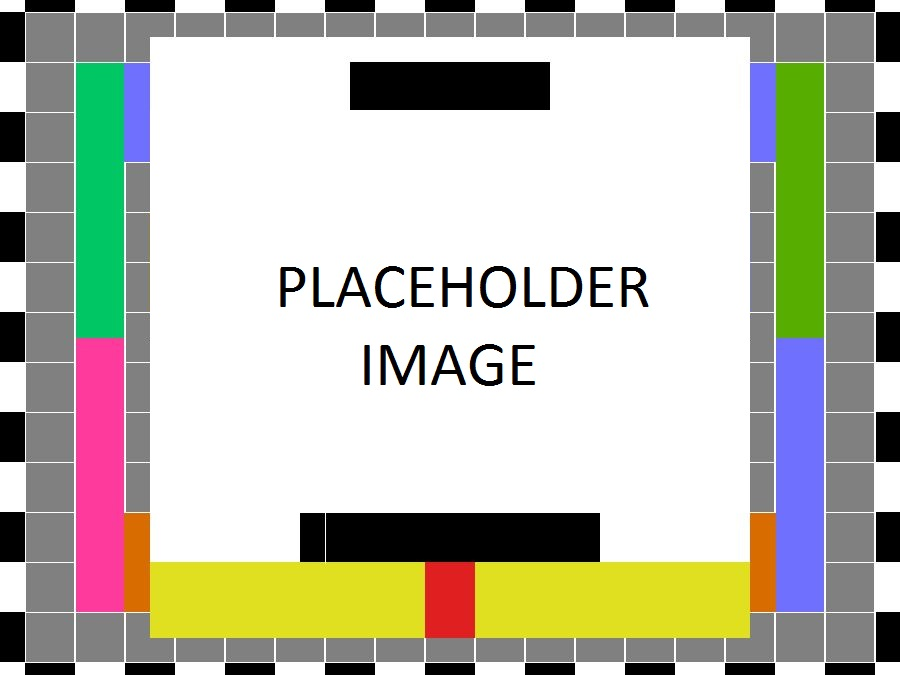
\includegraphics[width=0.60\textwidth]{images/test_image}
\end{figure}
\vspace{0.5 in}
{\centering \huge \color{accentcolor} \sc \textbf{\teamname \\ \productname} \par}
\vspace{0.5 in}
{\centering \large \sc \textbf{\authors} \par}
\newpage


%\vspace{1 in}
%\centerline{January 13th, 2012}
%\newpage

%%% Revision History
\begin{versionhistory}
  	\vhEntry{0.1}{09/20/24}{TP|MM|AT|SA}{document creation}
  	
\end{versionhistory}
\newpage

%%% Table of contents
\setcounter{tocdepth}{2}
\tableofcontents
\newpage

%%% List of figures and tables (optional)
\listoffigures
\listoftables
\newpage

%%% Document sections
\section{Introduction}
The laser harp is a novel musical instrument that utilizes laser beams to simulate the strings of a traditional harp. By interrupting these laser beams, users can produce corresponding musical notes, creating an engaging and interactive experience. This product is designed to be both educational and entertaining, aiming to inspire interest in STEM fields while providing a unique musical platform for enthusiasts and musicians.

\section{Product Concept}

The laser harp operates by projecting laser beams vertically from an array of laser emitters placed at the base. These beams are aligned with corresponding phototransistors positioned above, which detect the presence or absence of the laser light. When a user interrupts a laser beam by placing their hand in its path, the phototransistor detects the interruption and sends a signal to a microcontroller or a Raspberry Pi. The microcontroller processes this signal and triggers the playback of a pre-recorded musical note corresponding to the interrupted beam.

\section{Scope}

The scope of the laser harp project includes the design, development, and testing of a functional prototype that can demonstrate the key features and capabilities of the product. The project encompasses the following components:
\begin{itemize}
    \item \textbf{Laser and Phototransistor Array:} A set of laser emitters and phototransistors to detect beam interruptions.
    \item \textbf{Microcontroller/Raspberry Pi:} A processing unit to handle input signals from the phototransistors and control the audio output.
    \item \textbf{Audio System:} Speakers or an audio output interface to play the corresponding musical notes.
    \item \textbf{User Interface:} A simple and intuitive interface for calibration, instrument selection, pitch adjustment, octave control, and volume control.
    \item \textbf{Power Supply:} A reliable power source to ensure continuous operation of the laser harp.
\end{itemize}

\section{Key Requirements}

\begin{itemize}
    \item \textbf{Real-time Sound Playback:} The system must produce sound immediately upon the interruption of a laser beam, ensuring a responsive playing experience.
    \item \textbf{Multi-note Capability:} The laser harp should support the simultaneous interruption of multiple laser beams, allowing users to create chords.
    \item \textbf{User Interface:} A user-friendly interface for controlling various parameters such as instrument selection, pitch, octave, and volume.
    \item \textbf{Portability:} The device should be lightweight and easy to transport, making it suitable for demonstrations and performances in different locations.
    \item \textbf{Safety:} The lasers used must be Class 1 to ensure user safety, with no risk of direct eye exposure.
    \item \textbf{Power Supply:} The system should be powered by a reliable source, such as a rechargeable battery or an external power adapter, to ensure uninterrupted operation.
    \item \textbf{Durability:} The construction of the laser harp should be robust enough to withstand regular use and transportation.
\end{itemize}

By addressing these key requirements, the architectural design of the laser harp will focus on creating a functional, safe, and user-friendly musical instrument that can be used for both educational purposes and entertainment. The following sections will detail the specific design components, their interactions, and the overall system architecture to achieve the desired functionality and performance.

\section{System Overview}
Explain, at a high level, how you will implement a solution to the problem. Include a diagram of major components to the system (not a full architectural design, but a high level overview of the major system components and how a user or external system might interface). Avoid specific implementation details (operating system, programming languages, etc.). This section should occupy at least 1 full page.
\newpage
%\section{Subsystem Definitions \& Data Flow}
%This section breaks down your layer abstraction to another level of detail. Here you grapically represent the logical subsytems that compose each layer and show the interactions/interfaces between those subsystems. A subsystem can be thought of as a programming unit that implements one of the major functions of the layer. It, therefore, has data elements that serve as source/sinks for other subsystems. The logical data elements that flow between subsystems need to be explicitly defined at this point, beginning with a data flow-like diagram based on the block diagram.

\begin{figure}[h!]
	\centering
 	\includegraphics[width=\textwidth]{images/Subsystem}
 \caption{A simple data flow diagram}
\end{figure}

\newpage
\section{Input Layer Subsystems}
The input layer has four subsystems consisting of laser diodes for the strings, Dials for volume control, buttons for changing octaves, and instruments. The fourth input subsection is the touchscreen which has a graphical interface to do the same tasks but as a setup before playing.
\begin{figure}[h!]
	\centering
 	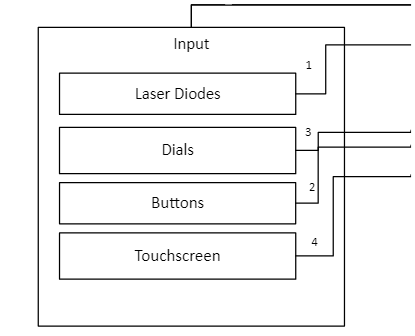
\includegraphics[width=0.60\textwidth]{images/InputSubsystem.png}
 \caption{Input Layer subsystems}
\end{figure}

\subsection{Input Subsystems}
The hardware involved in these subsystems are laser diodes and photo-transistors which read the interruptions of the laser diodes. The dial is a physical knob that is a potentiometer to control as a volume input for an onboard speaker.  Two buttons are working in a circular list to change the octaves of the harp sounds. One button is used as a way to change the instrument which also works as a circular list. 

\subsection{Input Operating System}
The operating system for this layer is driven by a Raspberry Pi operating system which handles all the inputs and outputs of each subsystem.

\subsection{Layer Software Dependencies}
A description of any software dependencies (libraries, frameworks, etc) required by the layer.

\begin{figure}[h!]
	\centering
 	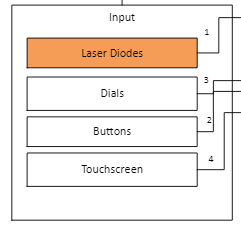
\includegraphics[width=0.60\textwidth]{images/Laserdiodes.png}
 \caption{Laser Diode Subsystem}
\end{figure}

\subsection{Laser Diodes}
This layer handles the input of the playing the harp as it is the harp's strings. The laser shines into the phototransistor at all times, when a finger blocks the laser the corresponding note is played. 


\subsubsection{Laser Diodes}
The laser diodes and phototransistors make up the hardware for the subsystem.

\subsubsection{Subsystem Operating System}
A description of any operating systems required by the subsystem.

\subsubsection{Subsystem Data Structures}
A description of any classes or other data structures that are worth discussing for the subsystem. For example, data being transmitted from a microcontroller to a PC via USB should be first be assembled into packets. What is the structure of the packets?

\subsubsection{Subsystem Data Processing}
A description of any algorithms or processing strategies that are worth discussing for the subsystem. If you are implementing a well-known algorithm, list it. If it is something unique to this project, discuss it in greater detail.


\begin{figure}[h!]
	\centering
 	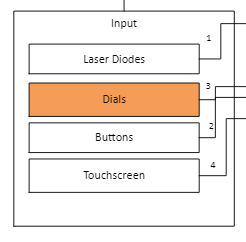
\includegraphics[width=0.60\textwidth]{images/Dials.png}
 \caption{Volume Control}
\end{figure}
\subsection{Volume Control}
This layer handles the input of a potentiometer to act as a volume control in conjunction with the GUI.


\subsubsection{Volume Control}
A single potentiometer will make up the hardware for this subsystem.

\subsubsection{Subsystem Operating System}
A description of any operating systems required by the subsystem.

\subsubsection{Subsystem Data Structures}
A description of any classes or other data structures that are worth discussing for the subsystem. For example, data being transmitted from a microcontroller to a PC via USB should be first be assembled into packets. What is the structure of the packets?

\subsubsection{Subsystem Data Processing}
A description of any algorithms or processing strategies that are worth discussing for the subsystem. If you are implementing a well-known algorithm, list it. If it is something unique to this project, discuss it in greater detail.

\newpage
\section{Control Unit Subsystems}
The Control Unit layer is responsible for processing input data, managing system logic, and generating output signals. The Control Unit includes sound settings, user settings, and a sound multiplexer.

\subsection{Layer Hardware}
The Control Unit layer uses a Raspberry Pi 4 as its primary hardware component.

\subsection{Layer Operating System}
This layer uses Raspberry Pi OS

\subsection{Layer Software Dependencies}
N/A

\subsection{Sound Setting}
The Sound Settings subsystem receives digital signals from the UserSettings and the Sound Settings subsystem is responsible for managing and applying the sound settings based on user input.

\begin{figure}[h!]
	\centering
 	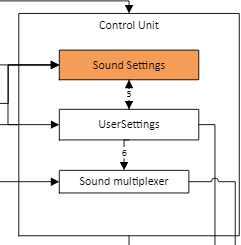
\includegraphics[width=0.60\textwidth]{architectural design specification latex/dds/detailed design specification latex/images/SoundSettings.png}
 \caption{Example subsystem description diagram}
\end{figure}

\subsubsection{Subsystem Hardware}
N/A

\subsubsection{Subsystem Operating System}
Raspberry pi OS    

\subsubsection{Subsystem Software Dependencies}
 N/A

\subsubsection{Subsystem Programming Languages}
 The subsystem uses Python for managing sound settings

\subsubsection{Subsystem Data Structures}
N/A

\subsubsection{Subsystem Data Processing}
N/A

\subsection{USerSetting}
The UserSettings subsystem is connected to the Sound Settings and the Sound Multiplexer subsystem

\begin{figure}[h!]
	\centering
 	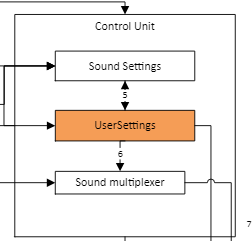
\includegraphics[width=0.60\textwidth]{architectural design specification latex/dds/detailed design specification latex/images/UserSettings.png}
 \caption{Example subsystem description diagram}
\end{figure}


\subsubsection{Subsystem Hardware}
N/A

\subsubsection{Subsystem Operating System}
Raspberry pi OS 

 \subsubsection{Subsystem Programming Languages}
 The subsystem uses Python for managing user settings

\subsubsection{Subsystem Data Structures}
N/A

\subsubsection{Subsystem Data Processing}
N/A

\subsection{Sound multiplexer.}
The Sound Multiplexer subsystem is connected to the Sound Settings subsystem and the Output Layer

\begin{figure}[h!]
	\centering
 	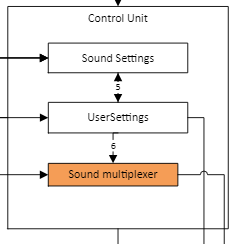
\includegraphics[width=0.60\textwidth]{architectural design specification latex/dds/detailed design specification latex/images/Soundmultiplex.png}
 \caption{Example subsystem description diagram}
\end{figure}

\subsubsection{Subsystem Hardware}
N/A

\subsubsection{Subsystem Operating System}
Raspberry pi OS

 \subsubsection{Subsystem Programming Languages}
 The subsystem uses Python for managing Sound multiplexer

\newpage
\section{Z Layer Subsystems}
In this section, the layer is described in terms of the hardware and software design. Specific implementation details, such as hardware components, programming languages, software dependencies, operating systems, etc. should be discussed. Any unnecessary items can be ommitted (for example, a pure software module without any specific hardware should not include a hardware subsection). The organization, titles, and content of the sections below can be modified as necessary for the project.

\subsection{Layer Hardware}
A description of any involved hardware components for the layer. For example, if each subsystem is a software process running on an embedded computer, discuss the specifics of that device here. Do not list a hardware component that only exists at the subsystem level (include it in the following sections).

\subsection{Layer Operating System}
A description of any operating systems required by the layer.

\subsection{Layer Software Dependencies}
A description of any software dependencies (libraries, frameworks, etc) required by the layer.

\subsection{Subsystem 1}
Descibe at a high level the purpose and basic design of this subsystem. Is it a piece of hardware, a class, a web service, or something else? Note that each of the subsystem items below are meant to be specific to that subystem and not a repeat of anything discussed above for the overall layer.

\begin{figure}[h!]
	\centering
 	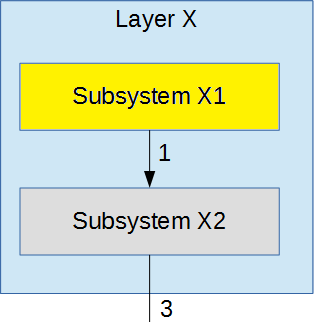
\includegraphics[width=0.60\textwidth]{images/subsystem}
 \caption{Example subsystem description diagram}
\end{figure}

\subsubsection{Subsystem Hardware}
A description of any involved hardware components for the subsystem.

\subsubsection{Subsystem Operating System}
A description of any operating systems required by the subsystem.

\subsubsection{Subsystem Software Dependencies}
A description of any software dependencies (libraries, frameworks, design software for mechanical parts or circuits, etc) required by the subsystem.

\subsubsection{Subsystem Programming Languages}
A description of any programming languages used by the subsystem.

\subsubsection{Subsystem Data Structures}
A description of any classes or other data structures that are worth discussing for the subsystem. For example, data being transmitted from a microcontroller to a PC via USB should be first be assembled into packets. What is the structure of the packets?

\subsubsection{Subsystem Data Processing}
A description of any algorithms or processing strategies that are worth discussing for the subsystem. If you are implementing a well-known algorithm, list it. If it is something unique to this project, discuss it in greater detail.



\newpage
\section{Appendix A}
Include any additional documents (CAD design, circuit schematics, etc) as an appendix as necessary.
\newpage

%%% References
\bibliographystyle{plain}
\bibliographystyle{reference/IEEEtran_custom}
\bibliography{reference/refs}{}

\end{document}
